\documentclass[11pt, oneside]{article}   	% use "amsart" instead of "article" for AMSLaTeX format
\usepackage{geometry}                		% See geometry.pdf to learn the layout options. There are lots.
\geometry{letterpaper}                   		% ... or a4paper or a5paper or ... 
\usepackage{graphicx}				% Use pdf, png, jpg, or eps§ with pdflatex; use eps in DVI mode
								% TeX will automatically convert eps --> pdf in pdflatex		
\usepackage{amssymb}
 
\usepackage[]{algorithm2e} 			% for the pseudocode

\date{}							% Activate to display a given date or no date
\parindent 0in
\parskip 6pt


 
\begin{document}

\title{\bf Gravity and Seismology }

\maketitle
 
%\section*{Learning Goals}
%In this lecture you will learn about:
%\begin{itemize}
%\item  
%\end{itemize}

 %------------------------------------------------------------------------------------------
\section*{Earth's Gravity}
%------------------------------------------------------------------------------------------
Precise measurements of variations in Earth's gravity field are used in the geosciences to map  geology and geologic processes over a range of spatial scales. Gravity measurements are sensitive to  lateral variations in rock density and so gravity surveys can be used to study the distribution of mass within Earth.  One of the earliest uses of gravity measurements was for prospecting for ore bodies, where metal oxide and sulphide minerals that are much denser than their host rocks  create excess gravity that can be measured with highly sensitive gravimeter instruments. Gravity  can be measured on the ground with small  sensors, but also can be made with airborne and satellite systems. Thus gravity data are used to study  mass anomalies arising from features as small as hidden tunnels and ore bodies to large scale features such as regional and continental scale tectonic structures. 

 The force of gravity that is exerted from one object onto another is described quantitively by Newton's law of universal gravitation. For two point masses $m_1$ and $m_2$, the force is
\begin{eqnarray}
	 \overrightarrow{F}=-G{\frac {m_{1}m_{2}}{r^{2}}} \hat r
\end{eqnarray}
where 
\begin{itemize}
\item  $ \overrightarrow{F}$ is the force applied on mass $m_2$ by mass $m_1$. Note that here the force is a vector, so it has both a magnitude and a direction. It's units are [N (Newtons) = kg m s$^{-2}$]
\item $G$ is the gravitational constant ($G=6.674\times10^{-11})$ [m$^3$ kg$^{-1}$s$^{-2}$]
\item $r$ is the distance between the centers of the two point masses [m].
\item  $\hat r$ is a unit vector pointing from $m_1$ to $m_2$.
\end{itemize}
Since $\hat r$ is the direction from $m_1$ to $m_2$, the negative sign means that the force $ \overrightarrow{F}$ is in the opposite direction from $m_2$ to $m_1$.
%
\begin{figure}[htbp]
\begin{center}
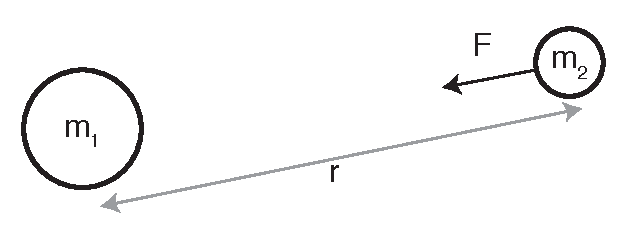
\includegraphics{masses.pdf}
\caption{Force of gravity exerted on mass $m_2$ due to mass $m_1$.}
\label{default}
\end{center}
\end{figure}
%

We also know from Newton's second law of motion is that the force is equal to the mass times its acceleration, or $F = ma$.  Equating the vector form of Newton's second law of motion with the formula above, and assuming the mass $m_1$ is the Earth's mass $m_e$, we can state
\begin{eqnarray}
	 \overrightarrow{F}=-G{\frac {m_{e}m_{2}}{r^{2}}} \hat r = m_2  \overrightarrow{a} = m_2  \overrightarrow{g}
	 \label{eq:Fg}
\end{eqnarray}
where we define the acceleration due to gravity as
\begin{eqnarray}
	 \overrightarrow{g}=-G{\frac {m_{e} }{r^{2}}} \hat r  
\end{eqnarray}
Given the Earth's mass $m_e = 5.976 \times 10^{24}$ kg and the equatorial radius $ r= 6.37816 \times 10^6$ m,  the acceleration from gravity is $g= 9.8$ m s$^{-2}$.

Given equation \ref{eq:Fg}, we can see that Earth's gravity will generate a force that is proportional to the mass $m_2$ being acted upon.  Since the mass of a body is simply the product of its density $\rho$ and volume $V$, we can say
\begin{eqnarray}
	 \overrightarrow{F}= m  \overrightarrow{g} = \rho V \overrightarrow{g} 
\end{eqnarray}
So for a fixed volume of material in Earth, its density is what controls the gravitational field produced by its volume.

Some densities of common materials in geology are shown in Table \ref{table:Densities}. The density of porous rocks will also increase with the degree of saturation, which is the amount of the pore space occupied by a fluid such as water or oil.

\begin{table}[htbp]
\caption{Densities of some rocks and minerals}
\begin{center}
\begin{tabular}{|c|c|}
\hline 
Material & Density $\rho$, kg m$^{-3}$ \\
\hline 
glacier ice &  917	\\
water & 1000 \\
silt & 1300-1800 \\
sandstone &  2000-2600\\
granite & 2600-2900 \\
basalt & 2800  \\
gabbro & 2800-3100\\ 
hematite, Fe$_2$O$_3$ & 5200\\
galena, PbS & 7500 \\
\hline 
\end{tabular}
\end{center}
\label{table:Densities}
\end{table}%

A formula for the gravitational acceleration of a sphere can be found through the application of Gauss' law for the flux through a  surface enclosing the sphere. The derivation  is a nice exercise in mathematical physics, but we don't have space for it here, so I will simply state the formula as:
\begin{eqnarray}
	 \overrightarrow{g}=-G{\frac {m }{r^{2}}} \hat r  =  -G{\frac {\rho V }{r^{2}}} \hat r 
\end{eqnarray}
where $m$ is the sphere's mass, $\rho$ is its density and $V$ is the volume.  This is precisely the same formula introduced earlier for a point mass. Thus we can see that the gravity  is {\it non-unique} with respect to the density and volume of the mass; so long as the product $\rho V$ is the same, the gravity anomaly will be the same.  

While the above formula is for the full gravity vector, it is most common to measure only the vertical component of gravity $g_z$, where $g_z =  |\overrightarrow{g}| \sin \theta$, as shown in Figure \ref{sphere}.  Further,  since gravity is produced by all the rocks in the ground, it is only the excess mass (or mass deficit) from the anomalous body that produces the change in  gravity. Thus we can replace $\rho$ above with the density contrast $\Delta \rho = \rho_{body} - \rho_{background}$. Since $\sin \theta  = z / r$ and $r = \sqrt{ x^2 + z^2}$, we have
 \begin{eqnarray}
	 g_z=   G{\frac {\Delta\rho V z}{r^{3}}}
\end{eqnarray}
Since the volume of the anomalous regions is $V = \frac{4}{3} \pi R^3$, the gravity {\it anomaly} above the spherical body is then
 \begin{eqnarray}
	 g_z=   G\Delta\rho \frac{4}{3} \pi R^3 {\frac { z}{(x^2 + z^2)^{3/2}}}
\end{eqnarray}
The anomaly for a cylinder (of infinite extent in the $y$ direction) has a similar (but slightly different) formula:
 \begin{eqnarray}
	 g_z=   G\Delta\rho 2 \pi R^2 {\frac { z}{x^2 + z^2}}
\end{eqnarray}

\begin{figure}[htbp]
\begin{center}
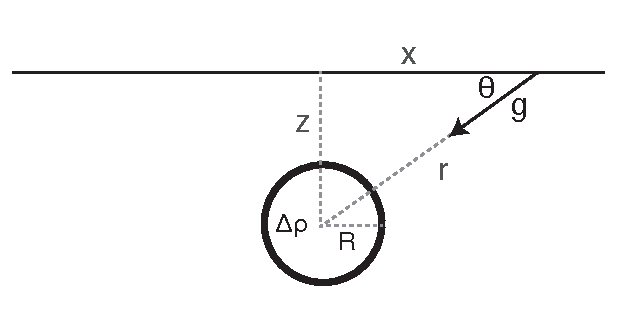
\includegraphics{sphere.pdf}
\caption{Geometry for a sphere or cylinder of radius $R$ and density anomaly $\Delta \rho$ with respect to the background geology.}
\label{sphere}
\end{center}
\end{figure}

\begin{figure}[htbp]
\begin{center}
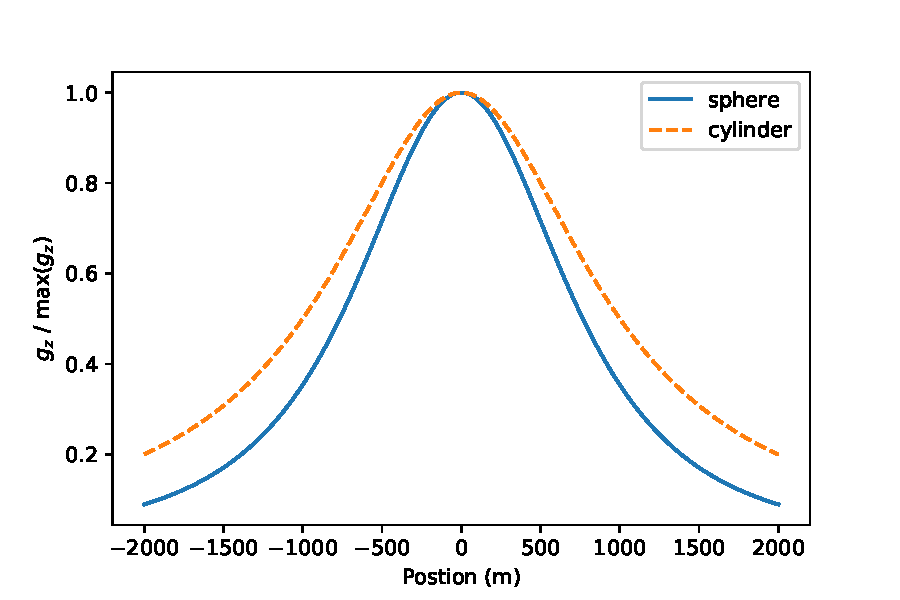
\includegraphics[width=0.75\textwidth]{cylinder_sphere.pdf}
\caption{Gravity anomalies for a sphere and cylinder of radius $R$ and anomalous density $\Delta \rho$.}
\label{sphere}
\end{center}
\end{figure}


 
\clearpage
%------------------------------------------------------------------------------------------
\section*{Seismology}
%------------------------------------------------------------------------------------------
 Seismology is the study of how elastic waves (i.e. ground motions) travel through Earth. When an earthquake or explosion occurs, it creates energy in the form elastic waves. If the energy is large enough, these seismic waves can be transmitted throughout the entire Earth. Thus, seismic waves are the best tool we have for studying the internal structure of our planet.  Here we will take a brief look at some of the fundamentals of how seismic waves so that you have enough information to complete the homework assignment. For a more detailed look at seismology (as well as some of the other topics we have cover in this course), consider taking  UN3201: Solid Earth Dynamics.
 
There are two fundamental types of seismic waves. P-waves, or compressional waves, involve motion in the direction that wave travels. S-waves, or secondary waves, have motion perpendicular to the direction of travel. P-waves can move through liquids (in the same way that sounds can be transmitted through water) whereas S-waves can only travel through solids.    We know that Earth's outer core is liquid because S-waves do not travel through it.  

P-waves and S-waves travel with different velocities, depending on the density and elastic moduli (the bulk and shear moduli) of the material they are moving through. In general the seismic velocity increases with depth in Earth due to increasing pressure and density.  

Ray theory is a branch of seismology where the seismic wave is approximated as a ray, which we will denote using arrows in the images below. A ray travels through a given medium with a velocity $v$.  The time that it takes to travel a given distance $h$ through a medium is simply $ t = h/v$.  Suppose we have a stack of layers with thickness $h_i$ and P-wave velocities $v_i$. The time for a P-wave that is normally incident on the layers (i.e., traveling vertically through them), is then:
\begin{eqnarray}
 t = \sum_{i=1}^n t_i = \sum_i^n \frac{h_i}{v_i} 
\end{eqnarray}
For example, consider the three layers in Figure \ref{layers}.  The time for  a ray traveling from the top to the bottom of the layers is 
\begin{eqnarray}
 t = t_1 + t_2 + t_3 = \frac{h_1}{v_1} +  \frac{h_2}{v_2} +  \frac{h_3}{v_3} 
\end{eqnarray}


\begin{figure}[htbp]
\begin{center}
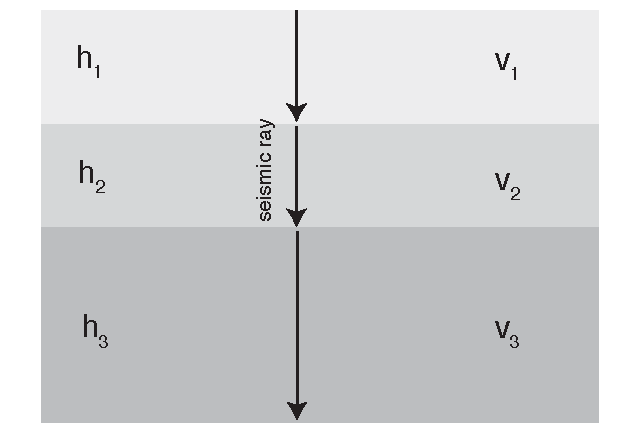
\includegraphics[width=0.7\textwidth]{seismic_layers.pdf}
\caption{Seismic ray traveling vertically through layers. }
\label{layers}
\end{center}
\end{figure}

For a ray that is incident upon a layer boundary at an angle, Snell's law shows how the transmitted ray angle will vary depending on the velocity of the two layers as well as the incidence angle:
\begin{eqnarray}
\frac{\sin(\theta_1)}{v_1} = \frac{\sin(\theta_2)}{v_2}
\end{eqnarray}

The transmitted wave is said to be {\it refracted}. A critically refracted wave occurs when $\theta_2 = 90$ degrees, meaning the refracted wave travels along the interface between the two layers. Since  $\theta_2 $ is known in this instance, the critical incidence angle can be found from Snell's law as:
\begin{eqnarray}
\frac{\sin(\theta_1)}{v_1} = \frac{1}{v_2}
\end{eqnarray}
or
\begin{eqnarray}
\theta_1 = \arcsin\left ( \frac{v_1}{v_2}\right )
\end{eqnarray}

The critically refracted wave travels with the velocity of the lower layer.

\begin{figure}[htbp]
\begin{center}
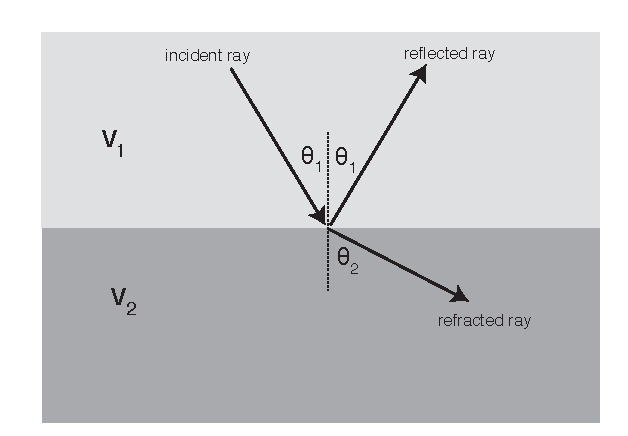
\includegraphics[width=0.7\textwidth]{SnellsLaw.pdf}
\caption{An incident seismic ray being reflected and refracted at a boundary where the velocity increases. }
\label{sphere}
\end{center}
\end{figure}



 
\end{document}  